\documentclass[11pt]{article}

\usepackage[a4paper,margin=1in]{geometry}
\usepackage[T1]{fontenc}
\usepackage[utf8]{inputenc}
\usepackage{lmodern}
\usepackage{microtype}
\usepackage{amsmath,amssymb,amsthm,mathtools}
\usepackage{booktabs,tabularx}
\usepackage{adjustbox}
\usepackage{enumitem}
\usepackage{graphicx}
% \usepackage[round,authoryear]{natbib}
\usepackage[numbers]{natbib}
\usepackage{xcolor}
\usepackage{hyperref}

\definecolor{linkblue}{RGB}{20,70,120}
\hypersetup{
  colorlinks=true,
  linkcolor=linkblue,
  citecolor=linkblue,
  urlcolor=linkblue,
  pdftitle={Two-Space Faithfulness in Projector-Based Self-Supervised Learning},
  pdfauthor={Anonymous Authors}
}
\urlstyle{same}

\setlength{\parindent}{1.2em}
\setlength{\parskip}{0pt}
\setlist[itemize]{leftmargin=*,topsep=3pt,itemsep=2pt}
\setlist[enumerate]{leftmargin=*,topsep=3pt,itemsep=2pt}
\numberwithin{equation}{section}

\newtheorem{theorem}{Theorem}[section]
\newtheorem{proposition}[theorem]{Proposition}
\newtheorem{corollary}[theorem]{Corollary}
\newtheorem{lemma}[theorem]{Lemma}
\theoremstyle{definition}
\newtheorem{definition}[theorem]{Definition}
\newtheorem{assumption}[theorem]{Assumption}
\theoremstyle{remark}
\newtheorem{remark}[theorem]{Remark}

\newenvironment{takeaway}
{\par\smallskip\noindent\begin{minipage}{\linewidth}\hrule\smallskip\textbf{Takeaway.}\ }
{\smallskip\hrule\end{minipage}\par\smallskip}

\newcommand{\TODO}[1]{\textcolor{red!70!black}{\textbf{TODO:} #1}}
\newcommand{\R}{\mathbb{R}}
\newcommand{\E}{\mathbb{E}}
\newcommand{\Pp}{\mathbb{P}}
\newcommand{\Cov}{\operatorname{Cov}}
\newcommand{\Var}{\operatorname{Var}}
\newcommand{\tr}{\operatorname{tr}}
\newcommand{\rank}{\operatorname{rank}}
\newcommand{\srank}{\operatorname{srank}}
\newcommand{\dist}{\operatorname{dist}}
\newcommand{\sign}{\operatorname{sign}}
\newcommand{\diag}{\operatorname{diag}}
\newcommand{\range}{\operatorname{range}}
\newcommand{\cM}{\mathcal{M}}
\newcommand{\cF}{\mathcal{F}}
\newcommand{\cL}{\mathcal{L}}
\newcommand{\cK}{\mathcal{K}}
\newcommand{\cE}{\mathcal{E}}
\newcommand{\norm}[1]{\lVert #1\rVert}
\newcommand{\ip}[2]{\langle #1,#2\rangle}
\newcommand{\argmin}{\operatorname*{arg\,min}}


\title{Two-Space Faithfulness in Projector-Based Self-Supervised Learning}
\author{Author Name}
\date{}


\begin{document}
\maketitle

\TODO{Title candidates: ? Method name: ? (Sec.~\ref{sec:method}).}

\begin{abstract}
Self-supervised methods train with a loss on a projected space \(Z\) and deploy the backbone representation \(H\). We show that the shape constraints these losses impose on \(Z\), such as Gaussianity, unit variance or isotropy, do not reach \(H\), both formally and on trained models. Maximal invariance is not the goal either: if it were, one would use \(Z\). We therefore define what \(H\) should keep beyond \(Z\) through augmentation thickness, the spread of one image's views relative to the spread between images, and show that it must be neither too small nor too large. Thickness also decides what a view-agreement objective keeps: directions in which views spread more than images are discarded, and feature learning makes the backbone follow the objective, so the backbone ends up narrow. We add a spectral conditioner on the backbone's per-image centers, derived from the layer-balance dynamics of two-layer networks, that gives every direction a lower bound on its variance while leaving the directions the loss uses shaped by the loss as before. Across seven self-supervised methods it raises the backbone's usable rank while training remains rich, and improves probes while thickness rises rather than falls, so the gain is not bought with invariance. Trained as a standalone objective on ImageNet-1k, the same picture holds from ViT-S to ViT-B and from 100 to 400 epochs, in linear probing, transfer and segmentation.
\end{abstract}

\section{Introduction}
\begin{itemize}
    \item The pipeline: \(H = f(V)\) for an augmented view \(V\), \(Z = p(H)\). The loss
    acts on \(Z\); downstream tasks use \(H\).

    \item \textbf{Claim 1.} The shape constraints these losses impose on \(Z\) do not reach \(H\).
    Formally, a loss that only sees \(Z\) cannot guarantee any property of \(H\) that a
    change of backbone and projector can undo. Measured: LeJEPA's Gaussianity, VICReg's
    unit variance and SimCLR's alignment hold at \(Z\) and fail at \(H\)
    (Fig.~\ref{fig:discrepancy}).

    \item \textbf{Claim 2.} Maximal invariance is not the goal either; otherwise one would deploy
    \(Z\). What \(H\) keeps beyond \(Z\) is augmentation thickness: how far one image's
    views spread, relative to how far images are from each other. Too little thickness
    removes distinctions that augmentations blur; too much makes single views noisy.
    Neither extreme is right.

    \item \textbf{Claim 3.} The objective keeps what it needs. A view-agreement loss uses the directions in which images differ more than their views do and feature learning aligns the backbone to the loss. The backbone therefore keeps the thin directions and loses the rest, which is exactly what a representation for unknown tasks should not lose. We show augmentation thickness is therefore a natural object to measure how much representations retain.

    \item \textbf{Claim 4.} We add a regularizer on the backbone's per-image centers that penalizes any direction whose variance vanishes. In a two-layer linear network we prove that the loss still shapes the directions it uses as before, while every other direction keeps a fixed variance instead of dying out: the term sets a lower bound.

    \item \textbf{Findings.} Added to seven existing methods, the term raises the backbone's usable
    rank two to five times while training remains rich, and improves linear and
    nearest-neighbor probes while thickness rises rather than falls. Used as
    a standalone objective on ImageNet-1k, the same picture holds from ViT-S to ViT-B and
    from 100 to 400 epochs, in linear probing, transfer and segmentation. We make no
    leaderboard claim.

    \item \textbf{Contributions:} (i) the two claims about \(Z\) and \(H\) with their measurements;
    (ii) thickness as the quantity that links what \(H\) should keep to what the objective
    removes; (iii) the regularizer, its derivation and the evidence.
\end{itemize}


\section{Related Work}

\subsection{Projection heads}
\begin{itemize}
    \item Why pre- and post-projector representations differ: expansion and shrinkage,
    feature reweighting, bottleneck, guillotine.
    \item Our position: none of these says what \(H\) should keep; Sec.~\ref{sec:what}
    does.
\end{itemize}

\subsection{Collapse and rank}
\begin{itemize}
    \item Variance and covariance terms at \(Z\) (VICReg, Barlow Twins, W-MSE, SIGReg);
    rank diagnostics (RankMe); encoder-side fixes (DirectCLR, WERank).
    \item Our position: the term is applied to the retained representation, on per-image
    centers, and is derived rather than posited.
\end{itemize}

\subsection{Feature learning}
\begin{itemize}
    \item Lazy and rich regimes; the balance between layers as the control knob; rich
    learning aligns features to the task in supervised settings. State these as
    supervised results.
    \item In self-supervised learning the same mechanism appears as dimensional collapse;
    cite the linear analyses.
    \item Our position: we want the rich regime without the alignment-driven loss of
    directions.
\end{itemize}


\section{What the retained representation should keep}\label{sec:what}

\subsection{Constraints on \(Z\) do not reach \(H\)}
\begin{itemize}
    \item In words: a loss that depends on the backbone and projector only through \(Z\)
    takes the same value on every pair that produces the same \(Z\). A property of \(H\)
    can be guaranteed by such a loss only if all those pairs share it. Coordinate changes,
    dropped information and added information all preserve \(Z\).
    \item Two explicit examples (appendix): a Gaussian \(Z\) with a non-Gaussian \(H\); a
    linearly separable \(Z\) with an XOR-shaped \(H\).
    \item This is not a failure of these methods. It says that a statement about \(Z\) is
    not yet a statement about \(H\).
\end{itemize}

\paragraph{Connection.}
The loss cannot say what \(H\) should be. We have to say it, and invariance is not the
answer.


\subsection{Invariance is not the goal: augmentation thickness}
\begin{itemize}
    \item For a space \(S \in \{H, Z\}\), split the covariance into the spread between
    image centers and the spread of one image's views,
    \[
        C_s = B_s + A_s,
        \qquad
        B_s = \Cov\big(\E[S \mid \text{image}]\big),
        \qquad
        A_s = \E\big[\Cov(S \mid \text{image})\big].
    \]

    \item Thickness is view spread measured against image spread,
    \[
        \Theta_h = B_h^{\dagger/2} A_h B_h^{\dagger/2},
        \qquad
        \text{along a direction } a:\ \frac{a^\top A_h a}{a^\top B_h a}.
    \]
    The same view spread means something different when images are far apart and when
    they are packed.

    \item What one view can tell about an image. Take any property of the image, a class
    or anything else. Two things limit how well it is read from a single augmented view. The
    augmentation sets one limit: if the views hide the evidence, no representation recovers
    it from one view. The representation sets the other: how well its image centers are
    arranged for that property, and how far the views spread around the centers along the
    direction used to read it.

    \item One identity (theorem; proof in the appendix). Error from a single view = error of
    the centers + view spread along the reading direction, and it is never below what the
    augmentation hides. Both sides of thickness are this one line.

    \item Too thin. A representation that is invariant along a direction cannot arrange its
    centers, along that direction, by anything the augmentation blurs. The invariant end,
    \(Z\), is where such distinctions are lost.

    \item Keeping a direction rearranges the centers (proposition). The objective drops
    directions by their view spread alone, blind to what their centers carry. Keep one of
    them and the image centers gain a coordinate: their arrangement improves by the class
    evidence that coordinate carries, and a single view collects that improvement discounted
    by the direction's thickness, never less than zero. This is how letting
    augmentation-sensitive information through improves the arrangement of the centers, and
    with it accuracy at \(H\).

    \item Too thick. The discount is the other side: a direction whose views spread far
    beyond the image spread adds little to a single-view read, however well its centers are
    arranged. Neither dropping such directions nor maximizing their spread is right.

    \item Reading: \(Z\) sits at the thin end by construction, and for every method its
    linear probe is below the backbone's. \(H\) should keep a moderate amount of view
    spread, not the least possible.
\end{itemize}

\paragraph{Connection.}
The constraints imposed on \(Z\) stay in \(Z\). What reaches \(H\) is the selection:
which directions survive. Training makes that selection by feature learning, and it reads
thickness to make it.


\subsection{Feature learning carries the selection from \(Z\) to \(H\)}
\begin{itemize}
    \item The loss wants few directions: those in which images differ more than their
    views do. It has no use for the rest.

    \item The backbone follows the loss. Features that stay near their initialization are
    called lazy; features that move to serve the loss are called rich, and deep networks
    train rich. In the two-layer linear model this is exact: the backbone puts variance
    \(s_i\) on each mode the loss uses and none on the others. In practice the untreated
    backbones in our zoo carry image-level variance in a fraction of their directions
    (Sec.~5).

    \item So \(H\) ends up thin where the loss looked and empty everywhere else.
    Sec.~3.2 argued against the first. The second is worse for a representation meant
    for unknown tasks: an empty direction cannot be read by any probe.

    \item We want to keep the first half of this, the backbone learning what the loss
    needs, and stop the second. The loss cannot help: it supervises \(H\) only through
    the few directions \(Z\) uses, and in the linear model no loss on \(Z\) can change
    how capacity is split between backbone and projector. What is missing is a target
    for every direction of \(H\). Sec.~\ref{sec:method} adds one and shows, in the
    linear model, that it leaves the learning of the needed directions untouched.
\end{itemize}

\begin{takeaway}
Training shapes \(H\) to \(Z\)'s needs through feature learning: thin where the loss
looked, empty elsewhere. A target on every direction of \(H\) keeps it broad.
\end{takeaway}


\section{A regularizer that keeps every direction}\label{sec:method}
\TODO{Method name. Candidates: dual-space spectral conditioning (DSC); backbone spectral
conditioning (BSC).}

\subsection{Two-layer linear network}
\begin{itemize}
    \item Setting: \(h = W_1 x\) (backbone), \(z = W_2 h\) (projector), and any loss
    \(\ell(W_2 W_1)\) that sees only the end-to-end map. The balance
    \(\Delta = W_2^\top W_2 - W_1 W_1^\top\) records which layer carries the scale.

    \item Conservation (lemma). Under gradient flow on any such loss, \(\Delta\) does not
    move. The loss never decides how much of the map lives in the backbone. This is the
    linear form of Sec.~3.1.

    \item The regularizer: weight decay on both layers plus a log-determinant on the
    backbone Gram,
    \[
        \frac{\lambda}{2}\big(\norm{W_1}_F^2 + \norm{W_2}_F^2\big)
        - \frac{\gamma}{2} \log\det\big(W_1 W_1^\top\big).
    \]

    \item Effect (proposition). \(\Delta\) now moves toward \(-cI\) with
    \(c = \gamma/\lambda\), at rate \(\lambda\), whatever the initialization and whatever
    the loss, because the loss terms cancel in the equation for \(\Delta\). The balance is
    chosen by the regularizer, not by the initialization.

    \item Allocation at the balanced solution (proposition). With \(s_i\) the singular
    values of the learned map, the backbone variance along mode \(i\) is
    \[
        a_i^2 = \tfrac12\Big(c + \sqrt{c^2 + 4 s_i^2}\Big).
    \]
    Two regimes in one formula: \(a_i^2 \approx s_i\) where the loss needs the mode
    (rich), \(a_i^2 \approx c\) where it does not. Every backbone direction keeps at least
    \(c\); nothing is frozen.

    \item \TODO{Figure: backbone variance per mode against \(s_i\) for the regularized
    network, the standard balanced network (\(a_i^2 = s_i\)) and a lazy network, plus
    feature drift over training. Replaces Figure\_1.png.}

    \item \TODO{State which regime \(\Delta = -cI\) corresponds to under the conventions
    of Domin\'e et al.\ and Kunin et al., and cite.}
\end{itemize}

\subsection{From weights to representations}
\begin{itemize}
    \item With whitened inputs the backbone Gram is the covariance of \(h\):
    \(W_1 W_1^\top = \Cov(h)\) and \(\norm{W_1}_F^2 = \tr \Cov(h)\). The regularizer is
    then a function of the representation only, which is what a nonlinear backbone lets
    us keep.

    \item Term used in practice,
    \[
        \cK(\mu, C)
        =
        \tfrac12\big(\norm{\mu}^2 + \tr C - \log\det C - d\big),
    \]
    the divergence of \(\mathcal N(\mu, C)\) from \(\mathcal N(0, I)\), computed on a
    random \(d'\)-dimensional slice of the representation at each step (appendix: slice,
    ring buffer, estimator).

    \item What it does: its minimizer is mean zero and identity covariance of the image
    centers, and it is two-sided: the log-determinant side punishes variance below one
    and diverges when a direction dies, the trace side punishes variance above one. With
    the agreement loss present, trained centers sit near that optimum, not at it.
\end{itemize}

\subsection{Centers, not views}
\begin{itemize}
    \item The mean of \(V\) views of one image has covariance \(B_s + A_s / V\).
    Conditioning per-image centers therefore asks for spread between images and only a
    \(1/V\) share of view spread. Sec.~3.2 says view spread should not be rewarded; this
    is how the method avoids it.

    \item Conditioning all views instead reads \(B_s + A_s\) and lets view spread pay for
    the term, in competition with the agreement loss over the same quantity.

    \item Objective:
    \[
        \cL
        =
        \cL_{\mathrm{agree}}(Z)
        + \lambda_z\, \cK\big(\hat\mu_z, \hat B_{z,V}\big)
        + \lambda_h\, \cK\big(\hat\mu_h, \hat B_{h,V}\big).
    \]
    The \(Z\) term is the anti-collapse term of the loss space and is a function of the
    end-to-end map; the \(H\) term is the new element and the one that pins the balance.

    \item Weights: the \(H\) term takes a few percent of the backbone gradient, the \(Z\)
    term about a third; procedure in the appendix.
\end{itemize}

\begin{takeaway}
One term, two places: at \(Z\) it prevents collapse of the loss space; at \(H\) it keeps
every backbone direction while the objective still shapes the ones it needs.
\end{takeaway}


\section{Experiments}

\subsection{Setup}
\begin{itemize}
    \item ImageNet-100, ViT-S/16, 100 epochs, one frame: seven methods (VICReg, SimCLR,
    BYOL, DINO, LeJEPA, VISReg, ours), each trained with and without the \(H\) term,
    everything else fixed.
    \item ImageNet-1k, ViT-S/16 and ViT-B/16, 100 and 400 epochs; one evaluation protocol
    for every row (linear probe and kNN); public checkpoints re-evaluated under it.
    \item One plain sentence for each quantity used below: usable rank (rank of the
    image-center covariance), thickness, center organization, feature drift.
\end{itemize}

\subsection{Constraints on \(Z\) do not reach \(H\)}
\begin{figure}[h]
  \centering
  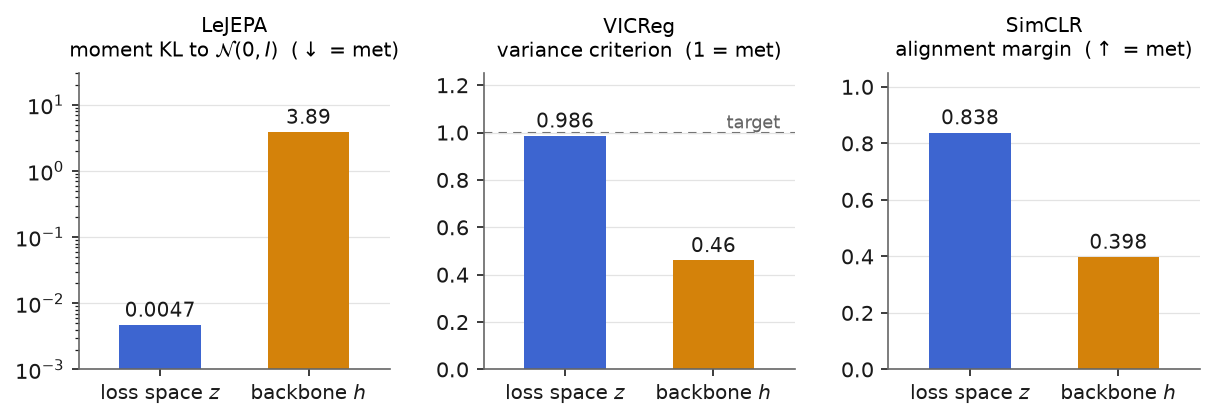
\includegraphics[width=0.75\linewidth]{figures/fig_discrepancy.png}
  \caption{Each method's own constraint, measured at \(Z\) and at \(H\) on the untreated
  models. \TODO{caption wording}}\label{fig:discrepancy}
\end{figure}

\subsection{The regularizer keeps capacity}
\begin{itemize}
    \item \TODO{Figure: \texttt{results/figures/paper/C2\_capacity.png} (and the
    across-training version C2b). Usable rank at \(H\) with and without the term, six
    pairs.}
    \item Point: every method gains, two to five times; the untreated models sit near what
    their loss needs.
\end{itemize}

\subsection{Learning is rich}
\begin{itemize}
    \item \TODO{Figure: \texttt{results/figures/e33\_feature\_drift.png} (raw until agreed).
    Feature drift from initialization and tangent-kernel alignment over training.}
    \item Point: features and the tangent kernel move far from initialization over
    training. The trained backbone is in the rich regime, not the lazy one.
\end{itemize}

\subsection{Thickness rises with the gain}
\begin{figure}[h]
  \centering
  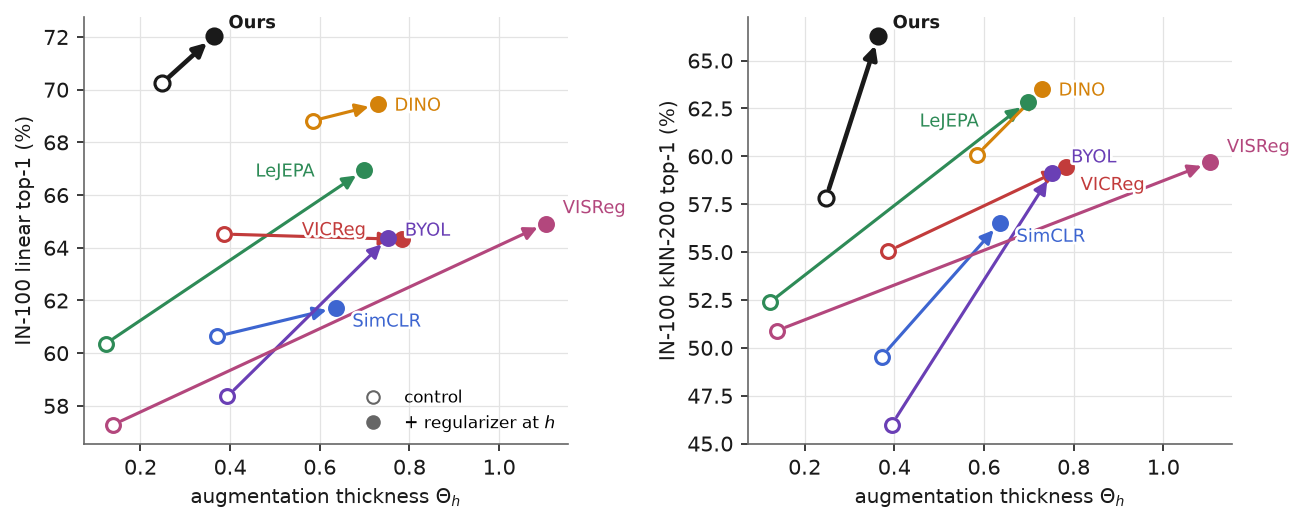
\includegraphics[width=0.85\linewidth]{figures/fig_treatment_arrows.png}
  \caption{Probe accuracy against thickness at \(H\), with and without the term.
  \TODO{caption wording}}\label{fig:arrows}
\end{figure}
\begin{itemize}
    \item In each model's own eigenbasis, the treated model has more directions that are
    both active and quiet, and a larger share of its class signal sits in them (E32;
    detail and figure in the appendix).

    \item Point: thickness rises moderately while accuracy rises, in every method. The
    gain is not bought with invariance.
\end{itemize}

\subsection{The picture holds at ImageNet-1k scale}
\begin{itemize}
    \item \TODO{Tables from \texttt{main.tex}: linear and kNN for ViT-S and ViT-B at 100
    and 400 epochs; transfer on eight datasets; ADE20k segmentation. ViT-L rows go to the
    appendix when they land.}
    \item The point is scaling, not ranking: the same objective, unchanged, from ViT-S to
    ViT-B and from 100 to 400 epochs. Public checkpoints appear for context only.
    \item One sentence on why the public rows are not a comparison: training data size,
    view sets, compute per epoch, recipes and epochs all differ.
\end{itemize}


\section{Limitations}
\begin{itemize}
    \item The theory is for a two-layer linear network; for deep networks it is a design
    principle, and the term regularizes activations rather than weights.
\end{itemize}


\section{Conclusion}
\begin{itemize}
    \item Constraints imposed at \(Z\) do not reach \(H\), and invariance is not what
    \(H\) is for.
    \item Thickness says what \(H\) should keep and explains what the objective removes;
    feature learning makes the backbone follow the objective.
    \item A regularizer derived from layer balance keeps every backbone direction while
    learning remains rich.
    \item It improves existing methods while thickness rises rather than falls, and as a
    standalone objective the same picture holds at ImageNet-1k scale.
\end{itemize}

% Appendix plan: proofs (non-identifiability, the two examples, the two-sided thickness
% theorem, balance conservation and dynamics, allocation); the quiet-core note (E32, figure
% results/figures/cloud_spread_zoo.png: directions counted in each model's own eigenbasis, quiet =
% small view spread relative to image spread rather than none; the class-energy share in the
% quiet core rises under the term); accessibility as the bridge
% diagnostic (C3, C3b); the fidelity law (C4);
% depth profiles (C7); trajectories (C6); the full treatment grid; the placement table
% and scatter; estimator and weighting details (slice, ring, shares); notes on the
% public baselines (recipes, data).

\end{document}
